%--------------------
% Packages
% -------------------
\documentclass[11pt,english]{article}
\usepackage{amsfonts}
\usepackage[left=2.5cm,top=2cm,right=2.5cm,bottom=3cm,bindingoffset=0cm]{geometry}
\usepackage{amsmath, amsthm, amssymb}
\usepackage{tikz}
\usetikzlibrary{calc}
\usetikzlibrary{decorations.pathreplacing,calligraphy}
\usepackage{fancyhdr}
%\usepackage{currfile}
\usepackage{nicefrac}
\usepackage{cite}
\usepackage{graphicx}
\usepackage{caption}
\usepackage{longtable}
\usepackage{rotating}
\usepackage{lscape}
\usepackage{booktabs}
\usepackage{float}
\usepackage{placeins}
\usepackage{setspace}
\usepackage[font=itshape]{quoting}
\onehalfspacing
\usepackage{mathrsfs}
\usepackage{tcolorbox}
\usepackage{xcolor}
\usepackage{subcaption}
\usepackage{float}
\usepackage[multiple]{footmisc}
\usepackage[T1]{fontenc}
\usepackage[sc]{mathpazo}
\usepackage{listings}
\usepackage{longtable}
\definecolor{cmured}{RGB}{175,30,45}
\definecolor{macroblue}{RGB}{56,108,176}
\usepackage[format=plain,
            labelfont=bf,
            textfont=]{caption}
\usepackage[colorlinks=true,citecolor=macroblue,linkcolor=macroblue,urlcolor=macroblue]{hyperref}
\usepackage{varioref}
\usepackage{chngcntr}
\usepackage{datetime}

\definecolor{darkgreen}{RGB}{30,175,88}
\definecolor{darkblue}{RGB}{30,118,175}
\definecolor{maroon}{rgb}{0.66,0,0}
\definecolor{darkgreen}{rgb}{0,0.69,0}

%Counters
\newtheorem{theorem}{Theorem}[section] 
\newtheorem{proposition}{Proposition}
\newtheorem{lemma}{Lemma}
\newtheorem{corollary}{Corollary}
\newtheorem{assumption}{Assumption}
\newtheorem{axiom}{Axiom}
\newtheorem{case}{Case}
\newtheorem{claim}{Claim}
\newtheorem{condition}{Condition}
\newtheorem{definition}{Definition}
\newtheorem{example}{Example}
\newtheorem{notation}{Notation}
\newtheorem{remark}{Remark}


\hypersetup{ 	
pdfsubject = {},
pdftitle = {TidyTuesday Week 38},
pdfauthor = {Pranay Gundam},
linkcolor= macroblue
}


\title{\textbf{TidyTuesday Week 38}}
\author{Pranay Gundam}


%-----------------------
% Begin document
%-----------------------
\begin{document}

\maketitle

\tableofcontents

\section{Weekly Summary}


\section{Date: 2024-09-18}
\noindent \textbf{Series ID: WPUDUR0211} 

\noindent This series is titled Producer Price Index by Commodity for Durability of Product: Durable Manufactured Goods (DISCONTINUED) and has a frequency of Monthly. The units are Index 1982=100 and the seasonal adjustment is Not Seasonally Adjusted.The observation start date is 1947-01-01 and the observation end date is 2018-12-01.The popularity of this series is 1. \\ 

\noindent \textbf{Series ID: MRTSMPCIM4423XUSN} 

\noindent This series is titled Retail Inventories: Furniture, Home Furnishings, Electronics, and Appliance Stores and has a frequency of Monthly, End of Period. The units are Percent Change from Preceding Period and the seasonal adjustment is Not Seasonally Adjusted.The observation start date is 1992-02-01 and the observation end date is 2024-07-01.The popularity of this series is 1. \\ 

\subsection{Regression Table}
\begin{center}
\begin{tabular}{lclc}
\toprule
\textbf{Dep. Variable:}          & value\_fred\_MRTSMPCIM4423XUSN & \textbf{  R-squared:         } &     0.003   \\
\textbf{Model:}                  &              OLS               & \textbf{  Adj. R-squared:    } &    -0.000   \\
\textbf{Method:}                 &         Least Squares          & \textbf{  F-statistic:       } &    0.8646   \\
\textbf{Date:}                   &        Wed, 18 Sep 2024        & \textbf{  Prob (F-statistic):} &    0.353    \\
\textbf{Time:}                   &            23:18:19            & \textbf{  Log-Likelihood:    } &   -959.15   \\
\textbf{No. Observations:}       &                323             & \textbf{  AIC:               } &     1922.   \\
\textbf{Df Residuals:}           &                321             & \textbf{  BIC:               } &     1930.   \\
\textbf{Df Model:}               &                  1             & \textbf{                     } &             \\
\textbf{Covariance Type:}        &           nonrobust            & \textbf{                     } &             \\
\bottomrule
\end{tabular}
\begin{tabular}{lcccccc}
                                 & \textbf{coef} & \textbf{std err} & \textbf{t} & \textbf{P$> |$t$|$} & \textbf{[0.025} & \textbf{0.975]}  \\
\midrule
\textbf{const}                   &       2.6034  &        2.489     &     1.046  &         0.296        &       -2.293    &        7.500     \\
\textbf{value\_fred\_WPUDUR0211} &      -0.0157  &        0.017     &    -0.930  &         0.353        &       -0.049    &        0.017     \\
\bottomrule
\end{tabular}
\begin{tabular}{lclc}
\textbf{Omnibus:}       & 53.368 & \textbf{  Durbin-Watson:     } &    1.585  \\
\textbf{Prob(Omnibus):} &  0.000 & \textbf{  Jarque-Bera (JB):  } &   93.834  \\
\textbf{Skew:}          & -0.928 & \textbf{  Prob(JB):          } & 4.21e-21  \\
\textbf{Kurtosis:}      &  4.877 & \textbf{  Cond. No.          } & 1.40e+03  \\
\bottomrule
\end{tabular}
%\caption{OLS Regression Results}
\end{center}

Notes: \newline
 [1] Standard Errors assume that the covariance matrix of the errors is correctly specified. \newline
 [2] The condition number is large, 1.4e+03. This might indicate that there are \newline
 strong multicollinearity or other numerical problems.

\subsection{Regression Plot}
\begin{figure}
\centering
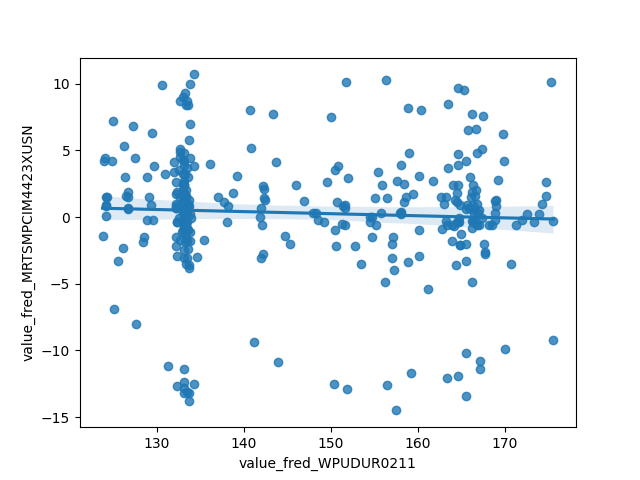
\includegraphics[scale = 0.9]{plots/plot_2024-09-18.png}
\caption{Regression Plot for 2024-09-18}
\end{figure}
\newpage

\section{Date: 2024-09-19}
\noindent \textbf{Series ID: CBLTCUSD} 

\noindent This series is titled Coinbase Litecoin and has a frequency of Daily, 7-Day. The units are U.S. Dollars and the seasonal adjustment is Not Seasonally Adjusted.The observation start date is 2016-08-17 and the observation end date is 2024-09-18.The popularity of this series is 14. \\ 

\noindent \textbf{Series ID: THREEFF8} 

\noindent This series is titled Fitted Instantaneous Forward Rate 8 Years Hence and has a frequency of Daily. The units are Percent and the seasonal adjustment is Not Seasonally Adjusted.The observation start date is 1990-01-02 and the observation end date is 2024-09-13.The popularity of this series is 1. \\ 

\subsection{Regression Tables and Plots}
\begin{center}
\begin{tabular}{lclc}
\toprule
\textbf{Dep. Variable:}        & value\_fred\_THREEFF8 & \textbf{  R-squared:         } &     0.002   \\
\textbf{Model:}                &          OLS          & \textbf{  Adj. R-squared:    } &     0.002   \\
\textbf{Method:}               &     Least Squares     & \textbf{  F-statistic:       } &     5.053   \\
\textbf{Date:}                 &    Thu, 19 Sep 2024   & \textbf{  Prob (F-statistic):} &   0.0247    \\
\textbf{Time:}                 &        11:31:03       & \textbf{  Log-Likelihood:    } &   -2624.6   \\
\textbf{No. Observations:}     &           2019        & \textbf{  AIC:               } &     5253.   \\
\textbf{Df Residuals:}         &           2017        & \textbf{  BIC:               } &     5265.   \\
\textbf{Df Model:}             &              1        & \textbf{                     } &             \\
\textbf{Covariance Type:}      &       nonrobust       & \textbf{                     } &             \\
\bottomrule
\end{tabular}
\begin{tabular}{lcccccc}
                               & \textbf{coef} & \textbf{std err} & \textbf{t} & \textbf{P$> |$t$|$} & \textbf{[0.025} & \textbf{0.975]}  \\
\midrule
\textbf{const}                 &       3.0640  &        0.035     &    88.434  &         0.000        &        2.996    &        3.132     \\
\textbf{value\_fred\_CBLTCUSD} &      -0.0008  &        0.000     &    -2.248  &         0.025        &       -0.001    &    -9.66e-05     \\
\bottomrule
\end{tabular}
\begin{tabular}{lclc}
\textbf{Omnibus:}       &  7.896 & \textbf{  Durbin-Watson:     } &    0.002  \\
\textbf{Prob(Omnibus):} &  0.019 & \textbf{  Jarque-Bera (JB):  } &    6.394  \\
\textbf{Skew:}          & -0.045 & \textbf{  Prob(JB):          } &   0.0409  \\
\textbf{Kurtosis:}      &  2.740 & \textbf{  Cond. No.          } &     180.  \\
\bottomrule
\end{tabular}
%\caption{OLS Regression Results}
\end{center}

Notes: \newline
 [1] Standard Errors assume that the covariance matrix of the errors is correctly specified.

\begin{figure}
\centering
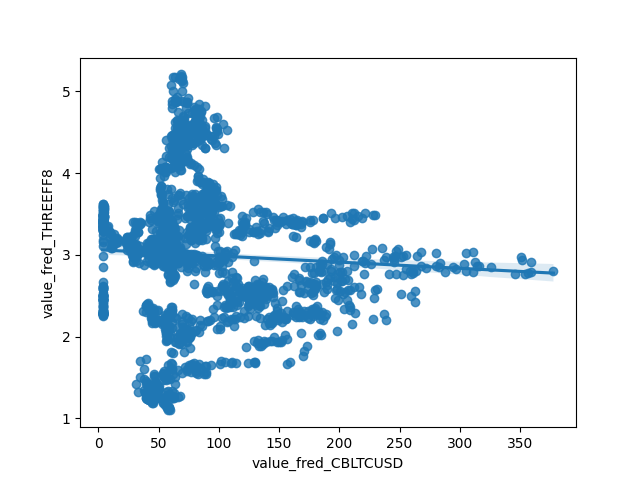
\includegraphics[scale = 0.9]{plots/plot_2024-09-19.png}
\caption{Regression Plot for 2024-09-19}
\end{figure}
\newpage

\section{Date: 2024-09-20}
\noindent \textbf{Series ID: G17MVSFLTRUCKS} 

\noindent This series is titled Regular Seasonal Factors: Light Truck Production and has a frequency of Monthly. The units are Seasonal Factor and the seasonal adjustment is Not Seasonally Adjusted.The observation start date is 1996-01-01 and the observation end date is 2025-06-01.The popularity of this series is 1. \\ 

\noindent \textbf{Series ID: PRGONUPIHCSA} 

\noindent This series is titled Medical Services Expenditures by Provider: Nursing Homes: Proprietary and Government Nursing Homes Price Index and has a frequency of Annual. The units are Index 2017=100 and the seasonal adjustment is Not Seasonally Adjusted.The observation start date is 2000-01-01 and the observation end date is 2021-01-01.The popularity of this series is 1. \\ 

\subsection{Regression Table}
\begin{center}
\begin{tabular}{lclc}
\toprule
\textbf{Dep. Variable:}              & value\_fred\_PRGONUPIHCSA & \textbf{  R-squared:         } &     0.002   \\
\textbf{Model:}                      &            OLS            & \textbf{  Adj. R-squared:    } &    -0.048   \\
\textbf{Method:}                     &       Least Squares       & \textbf{  F-statistic:       } &   0.04325   \\
\textbf{Date:}                       &      Fri, 20 Sep 2024     & \textbf{  Prob (F-statistic):} &    0.837    \\
\textbf{Time:}                       &          09:34:15         & \textbf{  Log-Likelihood:    } &   -90.742   \\
\textbf{No. Observations:}           &               22          & \textbf{  AIC:               } &     185.5   \\
\textbf{Df Residuals:}               &               20          & \textbf{  BIC:               } &     187.7   \\
\textbf{Df Model:}                   &                1          & \textbf{                     } &             \\
\textbf{Covariance Type:}            &         nonrobust         & \textbf{                     } &             \\
\bottomrule
\end{tabular}
\begin{tabular}{lcccccc}
                                     & \textbf{coef} & \textbf{std err} & \textbf{t} & \textbf{P$> |$t$|$} & \textbf{[0.025} & \textbf{0.975]}  \\
\midrule
\textbf{const}                       &      70.0979  &       81.638     &     0.859  &         0.401        &     -100.195    &      240.391     \\
\textbf{value\_fred\_G17MVSFLTRUCKS} &       0.1781  &        0.856     &     0.208  &         0.837        &       -1.608    &        1.964     \\
\bottomrule
\end{tabular}
\begin{tabular}{lclc}
\textbf{Omnibus:}       &  0.976 & \textbf{  Durbin-Watson:     } &    0.034  \\
\textbf{Prob(Omnibus):} &  0.614 & \textbf{  Jarque-Bera (JB):  } &    0.765  \\
\textbf{Skew:}          & -0.048 & \textbf{  Prob(JB):          } &    0.682  \\
\textbf{Kurtosis:}      &  2.091 & \textbf{  Cond. No.          } & 2.33e+03  \\
\bottomrule
\end{tabular}
%\caption{OLS Regression Results}
\end{center}

Notes: \newline
 [1] Standard Errors assume that the covariance matrix of the errors is correctly specified. \newline
 [2] The condition number is large, 2.33e+03. This might indicate that there are \newline
 strong multicollinearity or other numerical problems.

\subsection{Regression Plot}
\begin{figure}
\centering
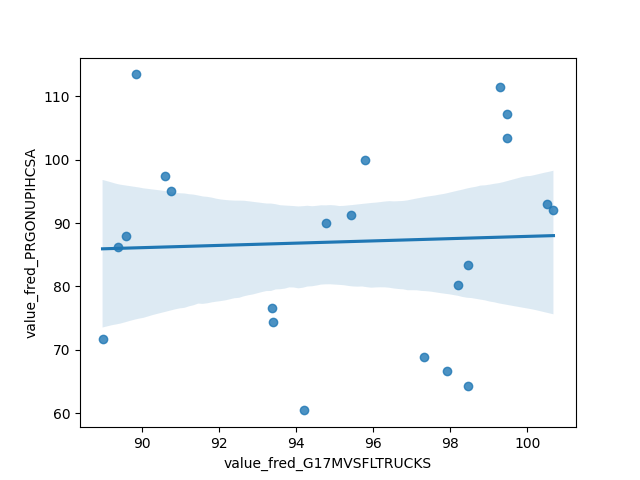
\includegraphics[scale = 0.9]{plots/plot_2024-09-20.png}
\caption{Regression Plot for 2024-09-20}
\end{figure}
\newpage

\section{Date: 2024-09-21}
\noindent \textbf{Series ID: MESTWHOLERQGSP} 

\noindent This series is titled Real Gross Domestic Product: Wholesale Trade (42) in the Mideast BEA Region and has a frequency of Quarterly. The units are Millions of Chained 2017 Dollars and the seasonal adjustment is Seasonally Adjusted Annual Rate.The observation start date is 2018-01-01 and the observation end date is 2024-01-01.The popularity of this series is 1. \\ 

\noindent \textbf{Series ID: CIU2013000100000I} 

\noindent This series is titled Employment Cost Index: Total compensation for Private industry workers in Manufacturing; management, professional, and related occupations and has a frequency of Quarterly. The units are Index Dec 2005=100 and the seasonal adjustment is Not Seasonally Adjusted.The observation start date is 2001-01-01 and the observation end date is 2024-04-01.The popularity of this series is 2. \\ 

\subsection{Regression Tables and Plots}
\begin{center}
\begin{tabular}{lclc}
\toprule
\textbf{Dep. Variable:}              & value\_fred\_CIU2013000100000I & \textbf{  R-squared:         } &     0.807   \\
\textbf{Model:}                      &              OLS               & \textbf{  Adj. R-squared:    } &     0.798   \\
\textbf{Method:}                     &         Least Squares          & \textbf{  F-statistic:       } &     96.07   \\
\textbf{Date:}                       &        Sat, 21 Sep 2024        & \textbf{  Prob (F-statistic):} &  1.11e-09   \\
\textbf{Time:}                       &            20:08:54            & \textbf{  Log-Likelihood:    } &   -62.766   \\
\textbf{No. Observations:}           &                 25             & \textbf{  AIC:               } &     129.5   \\
\textbf{Df Residuals:}               &                 23             & \textbf{  BIC:               } &     132.0   \\
\textbf{Df Model:}                   &                  1             & \textbf{                     } &             \\
\textbf{Covariance Type:}            &           nonrobust            & \textbf{                     } &             \\
\bottomrule
\end{tabular}
\begin{tabular}{lcccccc}
                                     & \textbf{coef} & \textbf{std err} & \textbf{t} & \textbf{P$> |$t$|$} & \textbf{[0.025} & \textbf{0.975]}  \\
\midrule
\textbf{const}                       &     255.8692  &       11.899     &    21.503  &         0.000        &      231.254    &      280.485     \\
\textbf{value\_fred\_MESTWHOLERQGSP} &      -0.0007  &     6.75e-05     &    -9.802  &         0.000        &       -0.001    &       -0.001     \\
\bottomrule
\end{tabular}
\begin{tabular}{lclc}
\textbf{Omnibus:}       & 20.224 & \textbf{  Durbin-Watson:     } &    2.138  \\
\textbf{Prob(Omnibus):} &  0.000 & \textbf{  Jarque-Bera (JB):  } &   30.570  \\
\textbf{Skew:}          & -1.624 & \textbf{  Prob(JB):          } & 2.30e-07  \\
\textbf{Kurtosis:}      &  7.336 & \textbf{  Cond. No.          } & 3.38e+06  \\
\bottomrule
\end{tabular}
%\caption{OLS Regression Results}
\end{center}

Notes: \newline
 [1] Standard Errors assume that the covariance matrix of the errors is correctly specified. \newline
 [2] The condition number is large, 3.38e+06. This might indicate that there are \newline
 strong multicollinearity or other numerical problems.

\begin{figure}
\centering
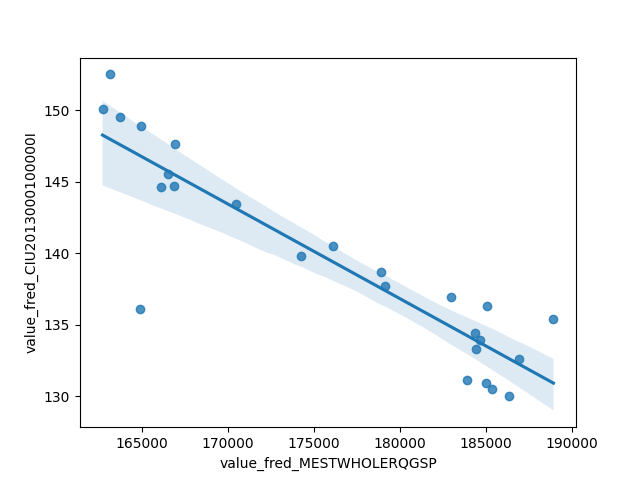
\includegraphics[scale = 0.9]{plots/plot_2024-09-21.png}
\caption{Regression Plot for 2024-09-21}
\end{figure}
\newpage

\section{Date: 2024-09-22}
\noindent \textbf{Series ID: DEINTDUSDDM} 

\noindent This series is titled German Intervention: Bundesbank Purchases on the Dollar/D-Mark (Millions of DEM) (DISCONTINUED) and has a frequency of Daily, 7-Day. The units are Millions of DEM and the seasonal adjustment is Not Seasonally Adjusted.The observation start date is 1976-01-02 and the observation end date is 1995-12-29.The popularity of this series is 2. \\ 

\noindent \textbf{Series ID: USGVDDNS} 

\noindent This series is titled U.S. Government Demand Deposits and Note Balances - Total (DISCONTINUED) and has a frequency of Monthly. The units are Billions of Dollars and the seasonal adjustment is Not Seasonally Adjusted.The observation start date is 1959-01-01 and the observation end date is 2021-01-01.The popularity of this series is 1. \\ 

\subsection{Regression Tables and Plots}
\begin{center}
\begin{tabular}{lclc}
\toprule
\textbf{Dep. Variable:}           & value\_fred\_USGVDDNS & \textbf{  R-squared:         } &     0.000   \\
\textbf{Model:}                   &          OLS          & \textbf{  Adj. R-squared:    } &    -0.004   \\
\textbf{Method:}                  &     Least Squares     & \textbf{  F-statistic:       } &    0.1184   \\
\textbf{Date:}                    &    Sun, 22 Sep 2024   & \textbf{  Prob (F-statistic):} &    0.731    \\
\textbf{Time:}                    &        15:34:40       & \textbf{  Log-Likelihood:    } &   -840.10   \\
\textbf{No. Observations:}        &            239        & \textbf{  AIC:               } &     1684.   \\
\textbf{Df Residuals:}            &            237        & \textbf{  BIC:               } &     1691.   \\
\textbf{Df Model:}                &              1        & \textbf{                     } &             \\
\textbf{Covariance Type:}         &       nonrobust       & \textbf{                     } &             \\
\bottomrule
\end{tabular}
\begin{tabular}{lcccccc}
                                  & \textbf{coef} & \textbf{std err} & \textbf{t} & \textbf{P$> |$t$|$} & \textbf{[0.025} & \textbf{0.975]}  \\
\midrule
\textbf{const}                    &      16.4059  &        0.530     &    30.930  &         0.000        &       15.361    &       17.451     \\
\textbf{value\_fred\_DEINTDUSDDM} &       0.0010  &        0.003     &     0.344  &         0.731        &       -0.005    &        0.007     \\
\bottomrule
\end{tabular}
\begin{tabular}{lclc}
\textbf{Omnibus:}       & 19.336 & \textbf{  Durbin-Watson:     } &    0.433  \\
\textbf{Prob(Omnibus):} &  0.000 & \textbf{  Jarque-Bera (JB):  } &    7.668  \\
\textbf{Skew:}          &  0.162 & \textbf{  Prob(JB):          } &   0.0216  \\
\textbf{Kurtosis:}      &  2.184 & \textbf{  Cond. No.          } &     185.  \\
\bottomrule
\end{tabular}
%\caption{OLS Regression Results}
\end{center}

Notes: \newline
 [1] Standard Errors assume that the covariance matrix of the errors is correctly specified.

\begin{figure}
\centering
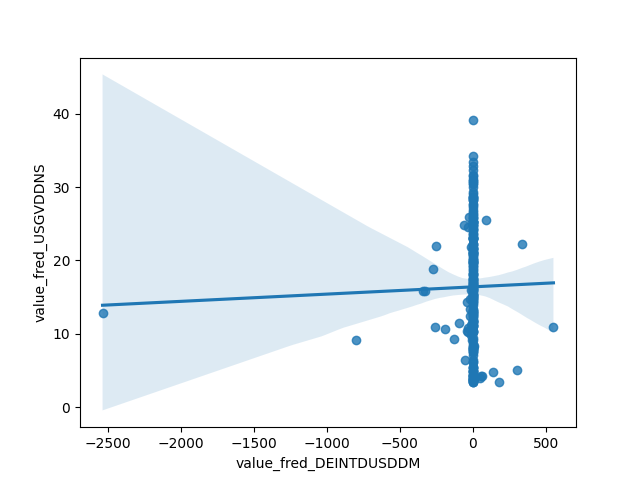
\includegraphics[scale = 0.9]{plots/plot_2024-09-22.png}
\caption{Regression Plot for 2024-09-22}
\end{figure}
\newpage


\end{document}
